\documentclass{ximera}

\newcommand{\RR}{\mathbb R}
\renewcommand{\d}{\,d}
\newcommand{\dd}[2][]{\frac{d #1}{d #2}}
\renewcommand{\l}{\ell}
\newcommand{\ddx}{\frac{d}{dx}}
\newcommand{\dfn}{\textbf}
\newcommand{\eval}[1]{\bigg[ #1 \bigg]}


\outcome{Find a tangent plane via the gradient.}

\begin{document}
\begin{exercise}
  Find an implicit equation for the tangent plane to the ellipsoid
  \[
  \frac{x^2}{12} +\frac{y^2}{6}+\frac{z^2}{4}=1
  \]
  \begin{image}
    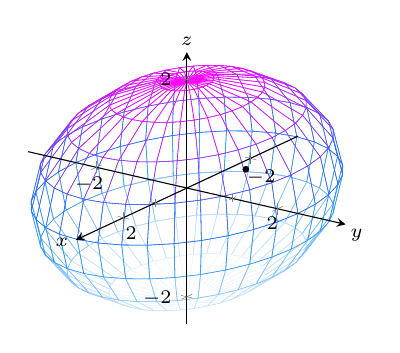
\begin{tikzpicture}
      \begin{axis}%
        [tick label style={font=\scriptsize},axis on top,
	  axis lines=center,
	  view={125}{25},
	  name=myplot,
	  %xtick=\empty,
	  %ytick={5},
	  %ztick={.7,-.7},
	  minor xtick=1,
	  minor ytick=1,
	  ymin=-3.5,ymax=3.5,
	  xmin=-3.5,xmax=3.5,
	  zmin=-2.5, zmax=2.5,
	  every axis x label/.style={at={(axis cs:\pgfkeysvalueof{/pgfplots/xmax},0,0)},xshift=-5pt,yshift=-1pt},
	  xlabel={\scriptsize $x$},
	  every axis y label/.style={at={(axis cs:0,\pgfkeysvalueof{/pgfplots/ymax},0)},xshift=4pt,yshift=-4pt},
	  ylabel={\scriptsize $y$},
	  every axis z label/.style={at={(axis cs:0,0,\pgfkeysvalueof{/pgfplots/zmax})},xshift=0pt,yshift=4pt},
	  zlabel={\scriptsize $z$},
          colormap/cool
	]

        \addplot3[domain=0:180,smooth,y domain=0:360,mesh,samples=19,samples y=19,very thin,z buffer=sort] ({cos(y)*(3.46*cos(x))},{cos(y)*(2.45*sin(x))},{2*sin(y)});
        
            
        \filldraw [black] (axis cs:1,2,1) circle (1pt);
      \end{axis}
    \end{tikzpicture}
  \end{image}
      Find the equation of the plane tangent to the ellipsoid at
      $\vec{p}$.
      \begin{prompt}
      \[
      \answer[given]{\frac{1}{6}(x-1) + \frac{2}{3}(y-2) + \frac{1}{2}(z-1)} = 0
      \]
      Use positive coefficients in your answer.
      \end{prompt}
\end{exercise}
\end{document}
